\documentclass[11pt,a4paper,openright,twoside]{extreport}
\usepackage[utf8]{inputenc}
\usepackage[english]{babel}
\usepackage[inner=1cm,outer=1cm,top=2cm,bottom=2cm]{geometry}
\usepackage{amsmath}
\usepackage{amsfonts}
\usepackage{textcomp}
\usepackage{amssymb}
\usepackage{pifont}
\usepackage{epstopdf}
\usepackage[singlespacing]{setspace}
\usepackage{tabularx}
\usepackage{mathrsfs}
\usepackage{rotating}
\usepackage{caption}
\usepackage[usenames,dvipsnames]{xcolor}
\usepackage{fancyref}
\usepackage{subcaption}
\usepackage{braket}
\usepackage{color}
\usepackage{float}
\usepackage{enumerate}
\usepackage[pagebackref]{hyperref}
\usepackage{afterpage}
\usepackage[makeroom]{cancel}

\usepackage{fancyhdr}
\pagestyle{fancy}

\usepackage{graphicx}
\usepackage{subcaption}
\usepackage{wrapfig}
\graphicspath{{images/}}

\usepackage{todonotes}

\fancyhead{}
\fancyhead[RE, LO]{{\nouppercase{\rightmark{Dhole, Mensing, Padalkar}}}}
\fancyhead[LE, RO]{\thepage}
\setlength{\headheight}{15pt}
\renewcommand{\headrulewidth}{0.4pt}

\fancyfoot{}
\fancyfoot[RE, LO]{{\nouppercase{\leftmark{MAS-SS18 | Hochschule Bonn-Rhein-Sieg}}}}
\fancyfoot[LE, RO]{Date: 03.05.2017}
\renewcommand{\footrulewidth}{0.4pt}

\hypersetup{
    pdftoolbar=true,        % show Acrobat’s toolbar?
    pdfmenubar=true,        % show Acrobat’s menu?
    pdffitwindow=false,     % window fit to page when opened
    pdfstartview={FitH},    % fits the width of the page to the window
    pdftitle={Scientific Experimentation and Evaluation Homework},    % title
    pdfauthor={Pranjal Dhole},     % author
    pdfsubject={Review},   % subject of the document
    pdfcreator={Pranjal Dhole},   % creator of the document
    pdfproducer={Pranjal Dhole}, % producer of the document
    pdfkeywords={SEEHomework} {Scientific Experimentation and Evaluation}, % list of keywords
    pdfnewwindow=true,      % links in new window
    colorlinks=true,       % false: boxed links; true: colored links
    linkcolor=MidnightBlue, % color of internal links (change box color with linkbordercolor)
    citecolor=Thistle,        % color of links to bibliography
    filecolor=magenta,      % color of file links
    urlcolor=Sepia           % color of external links
}

\newcommand{\sectionLine}{\begin{center}\line(1,0){500}\end{center}}
%%%%%%%%%%%%%%%%%%%%%%%%%%%%%%%%%%%%%%%%%%%%%%%%%%%%%%%%%%%%%%%%%%%%%%%%%%%
%specific
\raggedbottom
%%%%%%%%%%%%%%%%%%%%%%%%%%%%%%%%%%%%%%%%%%%%%%%%%%%%%%%%%%%%%%%%%%%%%%%%%%%
\pagenumbering{arabic}
\begin{document}
%%%%%%%%%%%%%%%%%%%%%%%%%%%%%%%%%%%%%%%%%%%%%%%%%%%%%%%%%%%%%%%%%%%%%%%%%%%
\begin{center}
\section*{\underline{Scientific Experimentation and Evaluation}}

\large{\textbf{Assignment 3: Statistical Evaluation}}\\
\large{Abhishek Padalkar, Max Mensing, Pranjal Dhole}\\
\large{Due date: Thursday, 03$^{\text{rd}}$ May, 2018}
\end{center}

\subsection*{Assignment 2}
\subsubsection*{1. Fix and, if necessary, rerun your experiment according to the feedback in class.}
We were not suggested to re-run the experiment.

\subsubsection*{2. Compare the observed and commanded motions: do they fit? if not, describe possible causes for this.}
\begin{itemize}
	\item \textbf{Straight Motion}
	
	\textbf{Commanded Motion}
	
	commanded speed = 18 cm/sec
	
	time = 2250 milliseconds
	
	expected distance to be traveled by by both wheels in x-axis direction = $ 18 * 2.25 = 40.5$ cm 
	
	expected distance to be traveled by by both wheels in x-axis direction = $0$ cm
	
	
	\textbf{Observed motion}
	
	mean distance traveled by right wheel in x-direction = 40.48 cm
	
	mean distance traveled by left wheel in x-direction = 40.3 cm 
	
	mean distance traveled by right wheel in y-direction = 0.055 cm 
	
	mean distance traveled by left wheel in y-direction = 0.075 cm 
	
	\item \textbf{Right Turn}
	
	\textbf{Commanded Motion} \newline
	Assume : \newline
	
	linear speed of right wheel = $v1$ \newline
	linear speed of left wheel = $v2$ \newline
	rotational speed of center of the axle of wheels = $\omega$ \newline
	commanded speed = 18 cm/sec \newline
	time = 2250 milliseconds \newline
	turn rate = 40 \newline
	distance between wheels (track width) = 14.5 cm 
	
		$$v1 = r1 * \omega$$
		$$v2 = (r1 + \text{track width} ) * \omega$$
		$$\omega = \frac{18 * 0.4}{14.5}$$
		$$\omega = 0.4966 \text{ rad/sec}$$
		$$r1 = 21.75$$
		$$W1x = \sin(0.4966 * 2.25) * 21.75 = 19.552 $$
		$$W1y = \cos(0.4966 * 2.25) * 21.75 - 1.75 = 9.52 - 1.75 = 7.77$$
	
		$$W2x = \sin(0.4966 * 2.25) * (21.75 + 14.5) = 32.58$$
		$$W2y = \cos(0.4966 * 2.25) * (21.75 + 14.5) - 1.75 = 15.87 - 1.75 = 13.13$$

	\item \textbf{Left Turn}
	
	Left turn is mirror motion of right turn, co-ordinates can be obtained by adding translations. 
	
	$$W2x = \sin(0.4966 * 2.25) * 21.75 = 19.552 $$
	$$W2y = \cos(0.4966 * 2.25) * 21.75 + 42.35 = 9.52 + 42.35 = 51.87$$
	
	$$W1x = \sin(0.4966 * 2.25) * (21.75 + 14.5) = 32.58$$
	$$W1y = \cos(0.4966 * 2.25) * (21.75 + 14.5) + 42.35 = 15.87 + 42.35 = 57.22$$
	
	
\end{itemize}

In case of straight line motion, the commanded motion matches with the observed motion. Small random error can be observed in the readings but it can be the result of inaccurate placement of robot before starting the run, inaccurate measurement or LED displacement. 

In case of turning motion, a large error can be observed. The facts for formula derivation for calculation of motion are taken from API provided by lejos library (\href{http://www.lejos.org/nxt/nxj/api/lejos/robotics/navigation/DifferentialPilot.html#steer(double)}{link}). This API documentation does not clarify the effect of turn rate used in \textit{steer} function well enough. The absolute speed value of outer wheel is not clarified. Hence it is assumed to be equal to absolute speed set by DifferentialPilot. This can be the cause of error.
Another reason of error can be the value of track width parsed in the code which is 18.6 cm but it is 14.5 cm on real robot.
If the formula provided in the documentation of lejos API for calculating speed of each wheel set by steer function considers outer wheel's speed equal to absolute speed set by DifferentialPilot function, then the error in track width value must not have any effect on experiment. But clearly, this is not the fact, the assumptions made on turn speed and steer function are needed to be revisited and made cleared with some other sources.      




\subsubsection*{3. Fit a Gaussian to your data and judge if the data is truly Gaussian or if it follows another distribution.}

\begin{figure}[ht]
\centering
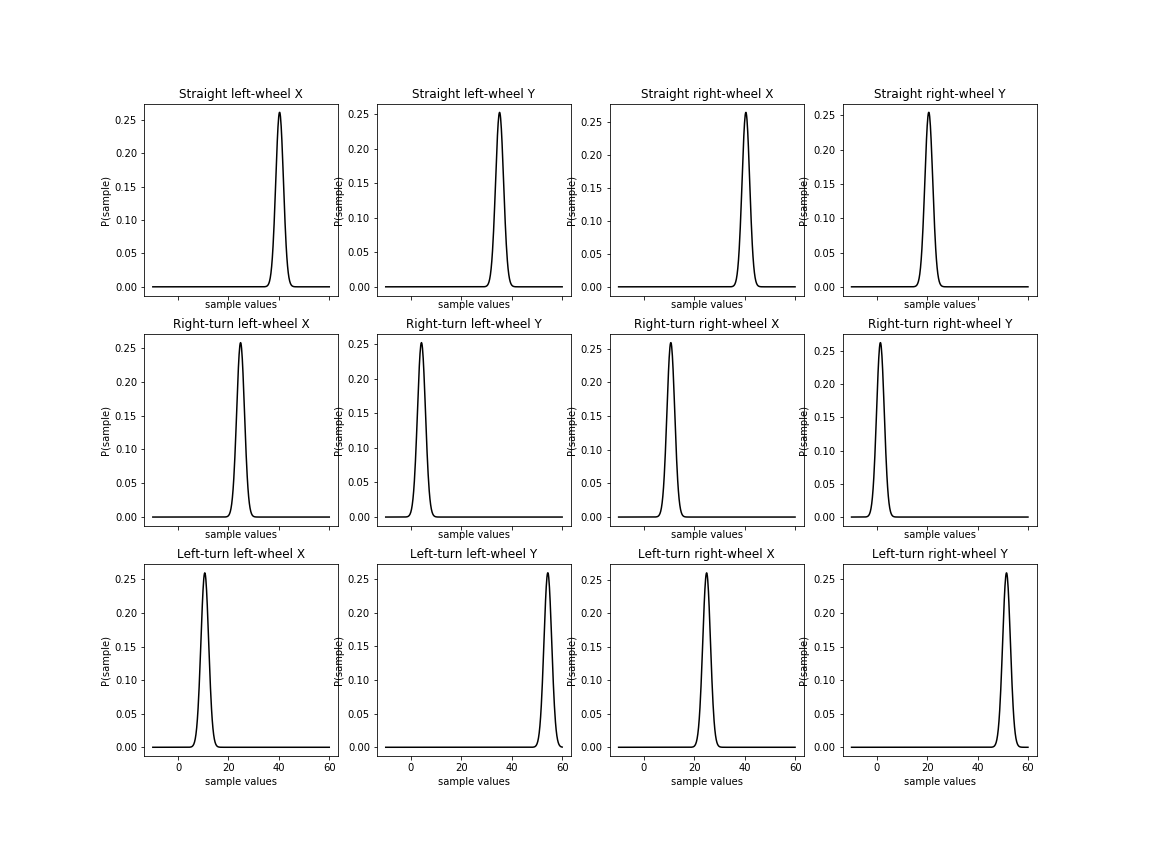
\includegraphics[width=\textwidth]{gaussian_fits.png}
\caption{Gaussian fit for the data using scikit-learn KernelDensity function}
\label{gaussian}
\end{figure}

\subsubsection*{4. Compare the estimated uncertainty of the measurement process itself with the statistical uncertainty of the observed end poses.}

\begin{table}[ht]
	\centering
	\begin{tabular}{| l | c | c | c | c | c | c |}
		\hline
		& \multicolumn{2}{c|}{left-turn motion} & \multicolumn{2}{c|}{ right-turn motion} & \multicolumn{2}{c|}{straight motion} \\
		\hline
		& right wheel & left wheel & right wheel & left wheel & right wheel & left wheel \\
		\hline
		Mean linear deviation $(\delta x, \delta y)$ cm & (0.1, 0.9) & (0.6, 0.8)
		& (0.7, 0.9) & (0.2, 0.9) & (0.5, 0.4) & 0.3, 0.4) \\
		\hline
		Mean ang. deviation ($\delta \theta$) degrees & 0.94 & 2.34 & 2.69 & 1.06 & 0.57 & 0.57 \\
		\hline
		$\sigma$ in final pose (x,y) cm & (0.3, 0.3) & (0.3, 0.3) & (0.3, 0.2) & (0.4, 0.5) & (0.2, 0.5) & (0.3, 0.5)\\
		\hline
		uncertainty in pose (x) cm & $(0.1 \pm 0.3)$ & $(0.6 \pm 0.3)$ & $(0.7 \pm 0.3)$ & $(0.2 \pm 0.4)$ & $(0.5 \pm 0.2)$ & $(0.3 \pm 0.3)$ \\
		uncertainty in pose (y) cm & $(0.9 \pm 0.3)$ & $(0.8 \pm 0.3)$ & $(0.9 \pm 0.2)$ & $(0.9 \pm 0.5)$ & $(0.4 \pm 0.5)$ & $(0.2 \pm 0.5)$ \\
		\hline
	\end{tabular}
	\caption{Statistical summary of robot motion}
	\label{stats}
\end{table}
There are three type of uncertainties which we estimated which can occur in the measurement. 
\begin{enumerate}
	\item Uncertainty in initial linear position of robot
	\item Uncertainty in initial angular position of robot
	\item uncertainty in measuring co-ordinates of the wheels
\end{enumerate}   

$1^{st}$ uncertainty will cause small linear error in measurement of wheel position equivalent to error in initial linear position.

$2^{nd}$ uncertainty will cause huge error in measurement of wheel position which will increase with distance traveled by robot. 

$3^{rd}$ uncertainty will cause small error (1 - 2 mm) in linear position of wheels.


\begin{table}[ht]
\centering
\begin{tabular}{| l | c | c | c | c | c | c |}
\hline
 & \multicolumn{2}{c|}{left-turn motion} & \multicolumn{2}{c|}{ right-turn motion} & \multicolumn{2}{c|}{straight motion} \\
\hline
 & right wheel & left wheel & right wheel & left wheel & right wheel & left wheel \\
\hline
Mean linear deviation $(\delta x, \delta y)$ cm & (0.1, 0.9) & (0.6, 0.8)
& (0.7, 0.9) & (0.2, 0.9) & (0.5, 0.4) & 0.3, 0.4) \\
\hline
Mean ang. deviation ($\delta \theta$) degrees & 0.94 & 2.34 & 2.69 & 1.06 & 0.57 & 0.57 \\
\hline
$\sigma$ in final pose (x,y) cm & (0.3, 0.3) & (0.3, 0.3) & (0.3, 0.2) & (0.4, 0.5) & (0.2, 0.5) & (0.3, 0.5)\\
\hline
uncertainty in final pose (x) cm & $(0.3 \pm 0.3)$ & $(0.6 \pm 0.3)$ & $(0.7 \pm 0.3)$ & $(0.4 \pm 0.4)$ & $(0.5 \pm 0.2)$ & $(0.3 \pm 0.3)$ \\
uncertainty in final pose (y) cm & $(0.9 \pm 0.3)$ & $(0.8 \pm 0.3)$ & $(0.9 \pm 0.2)$ & $(0.9 \pm 0.5)$ & $(0.5 \pm 0.5)$ & $(0.5 \pm 0.5)$ \\
\hline
\end{tabular}
\caption{Statistical uncertainty of observed end poses robot from observations.}
\label{stats}
\end{table}

\sectionLine
\subsection*{Deliverables 2}
Update your previous week’s report and add a description of the test for a match with a Gaussian distribution as well as a description of the observed differences between the observed and the computed motion and the actual and expected accuracy and precision. Include appropriate figures, diagrams, and images backing up any claims you make. The report must be self-contained and provide enough details to support any statement you make. If applicable, include a section on problems encountered. Your update should cover:

\subsubsection*{1. Any possible pre-processing of your data, like outlier detection and removal.}
We did not require any outlier detection algorithm since the data collection did not contain any outliers.

\subsubsection*{2. Fit of a Gaussian, either two individual ones in the x and y directions for each of the three cases or a proper two-dimensional distribution per case.}
We were able to fit the Gaussian to the data as shown in fig. \ref{gaussian}.

\subsubsection*{3. Check whether the data are actually distributed according to a Gaussian distribution.}
The data is too limited to conclude whether it comes from Gaussian distribution, however we were able to fit the data to a Gaussian distribution.

\subsubsection*{4. List of used software, including source of any function you wrote for performing your analysis.}
The software code is attached with the report.

\subsubsection*{5. An answer to the following question: When analysing the data with respect to the executed motions, which characteristic of the data do you establish here: the accuracy, the precision, or both?}

Because of the offset in the analytical calculations and actual mean of the readings, we can say that the executed motion was not accurate. But executed motion shows repeatability with lower variance, hence it can be concluded that the motion was precise. We will be revisiting our calculations by clearing the facts related to parameters used in the code, experiment will be re-performed if needed. In conclusion, with current calculations, turning motion was not accurate but it was precise. 
%%%%%%%%%%%%%%%%%%%%%%%%%%%%%%%%%%%%%%%%%%%%%%%%%%%%%%%%%%%%%%%%%%%%%%%%%%%%%
\end{document}